\chapter{HDMI}\label{chap:chap3}

Este capítulo descreve o trabalho realizado para cumprir a primeira parte do projeto: obter uma conexão HDMI entre recetor e transmissor. São descritas as várias configurações das placas HDMI disponiveis e ainda as arquiteturas desenvolvidas e implementadas para cumprir esta parte do projeto. 

\section{\textit{Hardware} utilizado}

Tal como mencionado no sub-capítulo \ref{sec:HDMIinFPGA}, para receber os dados provenientes do cabo HDMI e fazer a sua selecção são utilizadas duas placas HDMI (TB-FMCH-HDMI2 RX E TB-FMCH-HDMI2 TX) que, através das suas entradas e saída FMC de alta velocidade, conseguem enviar para a FPGA os sinais de imagem e som. Nas imagens \ref{fig:rx} e \ref{fig:tx} é possivel visualizar o recetor (TB-FMCH-HDMI2 RX) e o transmissor (TB-FMCH-HDMI2 TX) HDMI utilizados neste projeto. Em conjunto, estas duas placas são designadas apenas por TB-FMCH-HDMI2. Estas mesmas placas são constituidas por conectores HDMI, de seguida o sinal é enviado para um recetor ou transmissor HDMI, ADV7612 no caso do recetor e ADV7511 no caso do transmissor. Finalmente os sinais provenientes do recetor/transmissor são enviados para uma FGPA embebida na placa (XC6SLX45-3FGG484C) que, consoante a sua configuração, envia pelos conectores FMC os sinais de audio e video.

As placas possuem ainda uma PROM (\textit{Programmable read-only memory}) XCF16PFSG48C de configuração reprogramável que permite armazenar o \textit{bitstream} que configura a FPGA embebida do modo que se pretende. É esta FPGA embebida que em cada placa (RX e TX) é responsável pela selecção e envio dos dados pretendidos para os conectores FMC (e posterior envio para a FPGA), e como tal é necessário que estejam configuradas para realizarem tais procedimentos. O recurso a estas memórias reconfiguraveis vem permitir uma fácil alteração da configuração da FPGA uma vez que, segundo \cite{R026}, estas memórias de leitura permitem não só armazenar os \textit{bitstreams} de configuração da FPGA, mas também reconfigurá-los, caso se pretenda, de uma forma fácil e eficiente.

\subsection{Configurações da FPGA} \label{subsec:HDMIconfig}

A FPGA \textit{Spartan-6} (XC6SLX45-3FGG484C) embebida nas placas tem 3 configurações disponiveis. Estas configurações variam não só no suporte que têm, que pode ser apenasde imagem mas também de imagem e audio, mas variam também no número de bits por imagem que estas podem ter. Nas secções seguintes serão brevemente expostas as configurações disponiveis e como se pode tirar partido das mesmas no projeto.

--> Falar como é que se reconfigurou as placas
\subsubsection{Configuração por \textit{default}} \label{subsubsec:HDMIconfigdefault}

Esta configuração vem previamente escrita na memória PROM de fábrica e acaba por ser a mais simples de todas. Os dados enviados pelos conectores FMC são apenas referentes aos dados de imagem. As tabela \ref{table:HDMIdataRX} e \ref{table:HDMIdataTX} nas páginas \pageref{table:HDMIdataRX} e \pageref{table:HDMIdataTX} respectivamente identificam os pinos aos quais são atribuídas os sinais de dados de imagem HDMI tanto no recetor como no transmissor.

Esta configuração apenas transmite imagens RGB (\textit{Red Green Blue}) com 10 bits. Assim sendo, tal como referido em \cite{R009}, independentemente da formatação das imagens da fonte HDMI o recetor ADV7612 integrado na placa recetora HDMI converte a imagem para o formato RGB e transmite de maneira a enviar os dados em apenas 10 bits.  FALAR SOBRE ESTAS CONVERSÕES

A tabela \ref{table:HDMIdefaultSimplified} da página \pageref{table:HDMIdefaultSimplified}, adaptada de \cite{R009}, apresenta brevemente quais as portas das placas utilizadas e que sinais são transmitidos nas mesmas, no entanto é possivel encontrar na tabela \ref{table:HDMIdataDefaultdetail} do anexo \ref{ap1:HDMI} mais promenores relativamente a estes dados. Os nomes dos sinais são referentes aos sinais em TB-FMCH-HDMI2 (tanto TX como RX), assim como quando se faz referência à FPGA nestas tabelas estas correspondem às que estão embebidas nas placas HDMI. 

\begin{table}[h!]
	\centering
	\begin{tabular}{|c|c|c|c|}
		\hline
		\textbf{PIN}                                                                     & \textbf{FPGA -> FMC (RX)}                                                  & \textbf{FMC -> (TX)}                                                    & \textbf{Descrição}                                                      \\ \hline
		CLK0\_M2C\_P                                                                     & RX\#O\_LLC                                                                            & TX\#O\_DCLK                                                                           & \begin{tabular}[c]{@{}c@{}}Sinal de relógio dos\\   pixeis\end{tabular} \\ \hline
		LA00\_P\_CC                                                                      & RX\#0\_VSYNC                                                                          & TX\#0\_VSYNC                                                                          & \begin{tabular}[c]{@{}c@{}}Sincronização\\   Vertical\end{tabular}      \\ \hline
		LA01\_P\_CC                                                                      & RX\#0\_HSYNC                                                                          & TX\#0\_HSYNC                                                                          & \begin{tabular}[c]{@{}c@{}}Sincronização\\   Horizontal\end{tabular}    \\ \hline
		LA02\_P                                                                          & RX\#0\_DE                                                                             & TX\#0\_DE                                                                             & \begin{tabular}[c]{@{}c@{}}Sinal de \\ dados ativos\end{tabular}        \\ \hline
		\multirow{3}{*}{\begin{tabular}[c]{@{}c@{}}LA03\_P \\ a \\ LA32\_P\end{tabular}} & \multirow{3}{*}{\begin{tabular}[c]{@{}c@{}}RX\#0\_P0 \\ a \\ RX\#0\_P29\end{tabular}} & \multirow{3}{*}{\begin{tabular}[c]{@{}c@{}}TX\#0\_D0 \\ a \\ TX\#0\_D29\end{tabular}} & \multirow{3}{*}{Pixel de Imagem}                                        \\
		&                                                                                       &                                                                                       &                                                                         \\
		&                                                                                       &                                                                                       &                                                                         \\ \hline
	\end{tabular}
	\caption{Descrição e localização dos pinos de TB-FMCH-HDMI2 configurada por \textit{default}}
	\label{table:HDMIdefaultSimplified}
\end{table}

É de notar ainda que esta configuração é capaz de suportar até dois canais (RX0 e TX0, RX1 e TX1), no entanto nesta tabela apenas são apresentados os dados correspondentes ao canal 0 pois apenas será necessário utilizar um canal neste projeto. 

Apesar de ser um configuração simples, uma vez que apenas são transmitidos sinais de imagem em formato RGB, é uma configuração que será utilizada numa fase inicial em algumas arquiteturas implementadas que serão descritas no subcapitulo \ref{subsec:HDMIarquiteturas}.

\subsubsection{1 canal e suporte de audio} \label {subsubsec:HDMIconfig+audio}

Para além da configuração descrita anteriormente em \ref{subsubsec:HDMIconfigdefault} que apenas suporta a transmissão de imagem, existe ainda uma configuração capaz de suportar não só a transmissão de imagem mas também de som. A configuração que é escrita na PROM para programar a FPGA embebida controla o recetor ADV7612 de maneira a conseguir transmitir imagens no formato YCbCr ou RGB com 12 bits e também fazer a transmissão do audio em formato $I^{2}$S.

Assim como referido em \cite{R014}, neste caso a configuração da imagem está dependente da fonte HDMI, e é transmitida pelas placas tal como é emitida pela fonte, por outras palavras, se a fonte HDMI transmitir uma imagem em formato RGB é nesse formato que chega ao destino, no entanto se for transmitida uma imagem no formato YCbCr é nesse formato que chega ao seu destino. No caso do som, este é sempre transmitido em formato $I^{2}$S, o que implica a transmissão dos dados de audio mas também sinais de relógio necessários à sua transmissão. A tabela x passa a descrever com mais detalhe os sinais transmitidos para esta configuração da FPGA.

Na tabela \ref{table:HDMIaudiosuportSimplified} na página \pageref{table:HDMIaudiosuportSimplified} são brevemente apresentados as portas e os sinais usados com este tipo de configuração da FPGA embebida. Na tabela \ref{table:HDMI1canal+audioDETAIL} no anexo \ref{ap1:HDMI} é apresentada uma tabela semelhante a esta, mas que inclui mais detalhes relativamente aos pinos usados e ao seu uso. Ambas as tabelas foram adaptadas de \cite{R014} onde é são apresentados todos os detalhes dos conectores FMC das placas.

\begin{table}[h!]
	\centering
	\begin{tabular}{|c|c|c|c|}
		\hline
		\textbf{PIN}                                                                           & \textbf{FPGA -\textgreater FMC (RX)}                                                 & \textbf{FMC -> FPGA (TX)}                                                 & \textbf{FPGA->HDMI\_TX}                                                           \\ \hline
		CLK0\_M2C\_P                                                                           & RX\#0\_LLC                                                                           & TX\#0\_DCLK                                                                          & \begin{tabular}[c]{@{}c@{}}Sinal de relógio dos\\ pixeis\end{tabular}                        \\ \hline
		LA00\_P\_CC                                                                            & RX\#0\_VSYNC                                                                         & TX\#0\_VSYNC                                                                         & Sincronização vertical                                                                       \\ \hline
		LA01\_P\_CC                                                                            & RX\#0\_HSYNC                                                                         & TX\#0\_HSYNC                                                                         & Sincronização horizontal                                                                     \\ \hline
		LA02\_P                                                                                & RX\#0\_DE                                                                            & TX\#0\_DE                                                                            & Sinal de dados ativos                                                                        \\ \hline
		\multirow{3}{*}{\begin{tabular}[c]{@{}c@{}}LA03\_P\\   a LA32\_P\end{tabular}}         & \multirow{3}{*}{RX\#0\_P0 a RX\#0\_P29}                                              & \multirow{3}{*}{TX\#0\_D0 a TX\#0\_D29}                                              & \multirow{3}{*}{\begin{tabular}[c]{@{}c@{}}Pixel de imagem do bit\\   0 ao 29\end{tabular}}  \\
		&                                                                                      &                                                                                      &                                                                                              \\
		&                                                                                      &                                                                                      &                                                                                              \\ \hline
		\multirow{2}{*}{\begin{tabular}[c]{@{}c@{}}LA00\_N\_CC\\   a LA01\_N\_CC\end{tabular}} & \multirow{2}{*}{RX\#0\_InputVideoStatus}                                             & \multirow{2}{*}{TX\#0\_InputVideoStatus}                                             & \multirow{2}{*}{\begin{tabular}[c]{@{}c@{}}Formato de video\\   (2D/3D)\end{tabular}}        \\
		&                                                                                      &                                                                                      &                                                                                              \\ \hline
		LA19\_N                                                                                & RX\#0\_MCLK                                                                          & TX\#0\_MCLK                                                                          & \textit{Master Clock} de som                                                                          \\ \hline
		LA20\_N                                                                                & RX\#0\_SCLK                                                                          & TX\#0\_SCLK                                                                          & \textit{Serial Clock} de som                                                                          \\ \hline
		\multirow{2}{*}{\begin{tabular}[c]{@{}c@{}}LA21\_N\\   a LA26\_N\end{tabular}}         & \multirow{2}{*}{RX\#0\_AP0 a RX\#0\_AP5}                                             & \multirow{2}{*}{TX\#0\_AP0 a TX\#0\_AP5}                                             & \multirow{2}{*}{Dados de som}                                                                \\
		&                                                                                      &                                                                                      &                                                                                              \\ \hline
		\multirow{2}{*}{\begin{tabular}[c]{@{}c@{}}LA27\_N\\   a LA32\_N\end{tabular}}         & \multirow{2}{*}{\begin{tabular}[c]{@{}c@{}}RX\#0\_P30 a\\   RX\#0\_P35\end{tabular}} & \multirow{2}{*}{\begin{tabular}[c]{@{}c@{}}TX\#0\_P30 a\\   TX\#0\_P35\end{tabular}} & \multirow{2}{*}{\begin{tabular}[c]{@{}c@{}}Pixel de imagem do bit\\   30 ao 35\end{tabular}} \\
		&                                                                                      &                                                                                      &                                                                                              \\ \hline
	\end{tabular}
	\centering
	\caption{Descrição e localização dos pinos de TB-FMCH-HDMI2 configurada para 1 canal com suporte de audio}
	\label{table:HDMIaudiosuportSimplified}
\end{table}

Os dados referentes ao som transmitidos pela placa recetor HDMI e recebidos de seguida pela placa emissora HDMI estão mencionados com mais detalhe na tabela \ref{table:HDMI1canal+audioDETAIL}, e tal como indicado anteriormente, esta configuração é capaz de transmitir e receber dados no formato $I^{2}$S. Nas especificações deste protocolo, em \cite{R027}, são definidos os sinais transmitidos aquando a utilização deste formato, que passam a ser descritos:

\begin{enumerate}
	\item \textbf{\textit{Continuous Serial Clock} (SCK):} Este sinal é por vezes reconhecido pelo nome de \textit{Bit Clock} e é um sinal de relógio referente aos dados de som em série transmitidos pelos canais AP1, AP2, AP3 e AP4.
	
	\item \textbf{\textit{Word Select}(WS)}: Este sinal é por vezes também conhecido por \textit{Left/Right Clock} e é um sinal que indica o canal de som (esquerdo ou direito) que está a ser transmitido através dos dados em série recebidos ou enviados nas portas AP1, AP2, AP3 e AP4. É nomeado de sinal de relógio porque geralmente alterna entre 0 e 1 periodicamente, no entanto tal pode não acontecer, tal como referido em \cite{R027}. 
	
	\item \textbf{\textit{Serial Data}}: Sinais que transportam os dados de audio.

\end{enumerate}

Na imagem \ref{fig:i2s_audio} são ilustrados os sinais referentes ao audio descritos previamente. O sinal "SCLK" (\textit{Serial Clock}) é referente ao sinal "\textit{Continuous Serial Clock}", o sinal LRCLK (\textit{Left/Right Clock}) refere-se ao sinal "\textit{Word Select}" e ainda ISx refere-se ao sinal "\textit{Serial Data}".
	\begin{figure}[h!]
	\begin{center}
		\leavevmode
		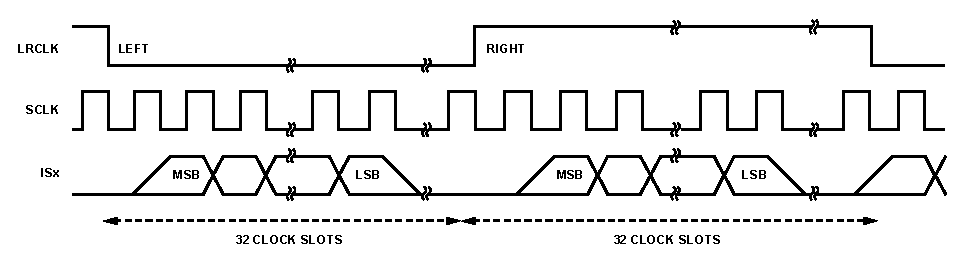
\includegraphics[width=1.0\textwidth]{audio_i2s}
		\caption{Ilustração dos sinais de som transmitidos no formato $I^{2}$S, retirada de \cite{R016}}
		\label{fig:i2s_audio}
	\end{center}
\end{figure}

Na placa recetora HDMI, que envia os dados para a FPGA Virtex-7, é também enviado o sinal \textit{Master Clock} que corresponde a um sinal de relógio de referência do sinais de audio da entrada e ainda dados de audio em AP0. É mencionado em \cite{R016} que estes dois sinais são referentes ao formato SPDIF e como tal não serão abordados neste projeto uma vez que as placas apenas suportam o formato $I^{2}$S.

Esta configuração das FPGAs embebidas nas placas é a configuração mais utilizada ao longo do projeto, uma vez que para além de ser versátil quanto ao formato das imagens transmitidas, é também capaz de suportar audio. Em contrapartida, apenas suporta um canal (ao contrário da anterior), mas tal não é um problema pois apenas se pretende obter uma transmissão num único canal entre dispositivo de fonte HDMI e dispositivo final HDMI. 


\subsubsection{2 canais melhorado} \label{subsubsec:HDMIconfigMelhorado}

--> Dizer que esta configuração faz tal tal e tal, mas que não será abordad uma vez que nao foi utilizada

\subsection{Configuração dos \textit{switches}}

Explicar como configurar os switches para obter o que queremos

\subsection{Arquiteturas Desenvolvidas} \label{subsec:HDMIarquiteturas}

Neste sub-capitulo passam a ser descritas as arquiteturas desenvolvidas e implementadas na FPGA referentes à comunicação entre as placas HDMI.  Por outras palavras, é feita uma aplicação daquilo que foi explicado sobre as placas HDMI a serem utilizadas até agora em arquiteturas implementadas e testadas em FPGA.

\subsubsection{Transmissão de uma imagem gerada na FPGA}

Numa fase inicil do projeto, optou-se por simplificar a transmissão e para tal utilizou-se apenas a placa transmissora HDMI configurada por defeito. Contrui-se em Verilog um bloco capaz de gerar uma imagem para ser transmitida, mais especificamente uma barra de cores, e utlizou-se essa imagem para ser transmitida pelos conectore FMC.

O bloco gerador de uma barra de cores foi adaptado de um bloco disponibilizado pela \textit{Inrenvium} aquando a compra das placas. Apesar de ter sido ligeiramente adaptado para este caso em especifico, este baseia-se essencialmente numa maquina de estados que vai contando as linhas e as colunas para que possa enviar não só os valores das cores de cada pixel, mas também os sinais de controlo como a sincronização vertical, a sincronização horizontal e ainda os valor de pixeis ativos.

Para que se entenda mais facilmente como e quando se transmitem os sinais de controlo da imagem e também os valor dos pixeis é demonstrado na imagem \ref{fig:colorBar_exemple} na página \pageref{fig:colorBar_exemple} uma exemplo de transmissão de uma imagem gerada na FPGA. Antes de passar para descrição da geração da imagem passam a ser descritos os acrónimos apresentados na figura:

\begin{enumerate}
	\item \textbf{HRES:} \textit{Horizontal Resolution} é o parâmetro que define a resolução horizontal da imagem que vai ser gerada pelo bloco, ou seja o número de pixeis em cada linha de transmissão.
	\item \textbf{HSW:} \textit{Horizontal Sync Width} é o parâmetro que define o número de ciclos de relógio que o sinal de sincronização horizontal tem.
	\item \textbf{HBP:} \textit{Horizontal Back Porch} é o parâmetro que define o número de pixeis que não contêm informação útil (relativamente à cor dos mesmos) antes de começar a ser transmitida a linha de imagem.
	\item \textbf{HFP:} \textit{Horizontal Front Porch} é o parâmetro que define o número de pixeis que não contem informação útil depois de ser transmitida uma linha da imagem.
	\item \textbf{VRES:} \textit{Vertical Resolution} é o parâmetro que define a resolução vertical da imagem que vai ser gerada pelo bloco, por outras palavras é o número de linhas de pixeis a ser geradas.
	\item \textbf{VSW:} \textit{Vertical Sync Width} é o parâmetro que define o número de linhas horizontais que o sinal de sincronização vertical está ativo.
	\item \textbf{VBP:} \textit{Vertical Back Porch} é o parâmetro que define o número de linhas horizontais que não contém informação útil relativamente ao pixeis antes de começarem a ser transmitidas as linhas de pixeis.
	\item \textbf{VFP:} \textit{Vertical Front Porch} é o parâmetro que define o número de linhas horizontais que não contém informação útil relativamente ao pixeis depois de terem sido transmitidas todas as linhas horizontais da imagem.
\end{enumerate}
	
\begin{figure}[h!]
	\begin{center}
		\leavevmode
		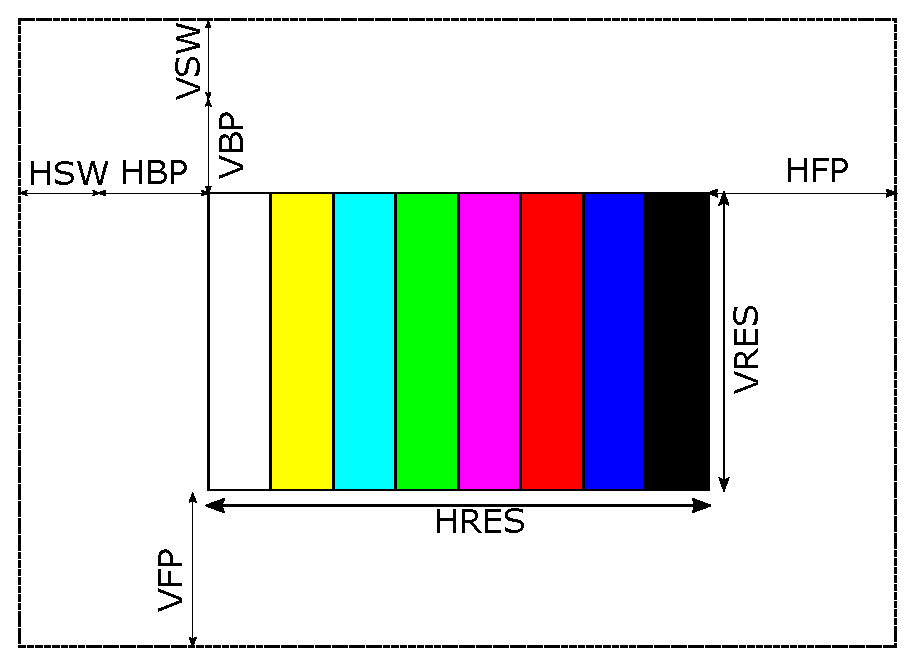
\includegraphics[width=1.0\textwidth]{exemplo_colorBar}
		\caption{Exemplo de imagem gerada pelo modulo desenvolvido}
		\label{fig:colorBar_exemple}
	\end{center}
\end{figure}

Para gerar uma imagem em \textit{FULL HD} cuja resolução é 1920x1080 pixeis e o sinal de relógio deve ter uma frequência de 148.5 MHz, foram o utilizados os seguintes valores para os parâmetro previamente descritos: HRES = 1920, HSW = 44, HBP = 44, HFP = 148,  VRES = 1080, VSW = 5, VBP = 36 e VFP = 4.
%
%\begin{itemize}
%	\item HRES = 1920
%	\item HSW = 44
%	\item HBP = 44
%	\item HFP = 148
%	\item VRES = 1080
%	\item VSW = 5
%	\item VBP = 36
%	\item VFP = 4
%\end{itemize}

A figura \ref{fig:colorBar_fsm} na página \pageref{fig:colorBar_fsm} ilustra a maquina de estados desenvolvida para implementar a geração de uma barra a cores na FPGA. 

\begin{figure}[h!]
	\begin{center}
		\leavevmode
		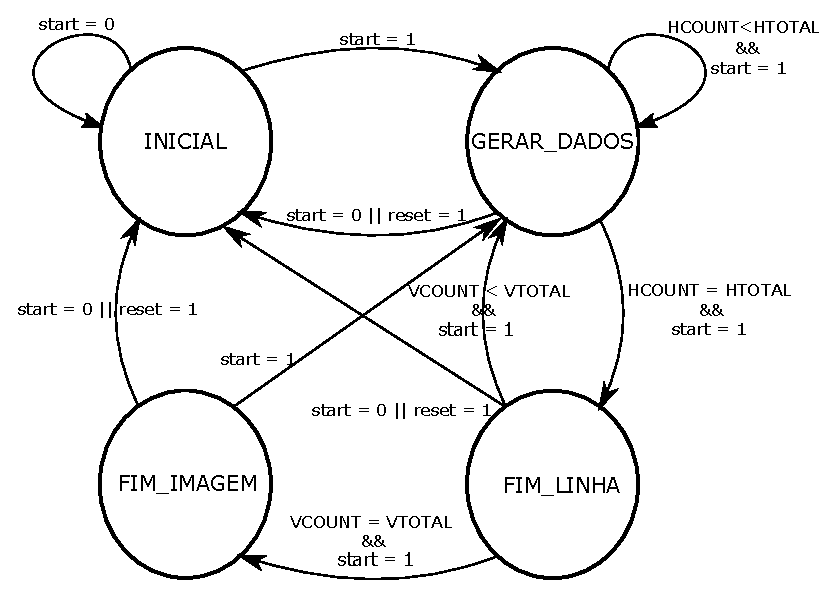
\includegraphics[width=1.0\textwidth]{colorBar_FSM}
		\caption{Máquina de estados para gerar uma barra de cores}
		\label{fig:colorBar_fsm}
	\end{center}
\end{figure}

Os registos VCOUNT E HCOUNT de decisão que se visualiza na figura correspondem a contadores que vão contanto pixel a pixel até ao fim de uma linha (no caso do HCOUNT) ou então de uma imagem inteira (no caso do VCOUNT). Os valores de HTOTAL e VTOTAL não são mais do que a soma de todo o tamanho dos dados na horizontal e na vertical respectivamente. Assim sendo, para este caso em especifico obtem-se os seguintes valores:
\begin{itemize}
	\item HTOTAL = HSW + HBP + HRES + HFP = 44 + 44 + 1920 + 148 = 2156
	\item VTOTAL = VSW + VBP + VRES + VFP = 5 + 36 + 1080 + 4 = 1125
\end{itemize}

Para além destes sinais de decisão para mudança de estado existem mais dois sinais no diagrama da máquina de estados presente na figura \ref{fig:colorBar_fsm} que ainda não foram mencionados que são o \textit{reset} e o \textit{start}. Estes dois sinais são botões do utilizador que lhe permitem definir quando se pretende que a transmissão esteja ativa ou desativa (através do botão \textit{start}) ou então quando se pretende restabelecer os dados originais da máquina de estados (através do botão \textit{reset}). 


Existem 4 estados nesta máquina eu consistem essencialmente em detecção do final de uma linha, e detecção do final de uma imagem e geração de dados. Os estados passam a ser descritos de seguida:

\begin{enumerate}
	\item \textbf{Estado inicial:} Neste estado são configurados os parâmetros para o inicio de uma transmissão, ou seja, os valores de HCOUNT e VCOUNT são igualados ao valor total do tamanho na horizontal e na vertical respectivamente. Por outras palavras, os valores de HCOUNT e VCOUNT são igualados a HTOTAL e VTOTAL respectivamente. Isto acontece porque é possivel retornar a este estado estando em qualquer um dos outros desde que seja pressionado o botão  de \textit{reset} ou então que a transmissão seja desligada pelo utilizador (\textit{start} = 0).
	\item \textbf{Estado para gerar dados:} Neste estado, ao flanco positivo do sinal de relógio do sistema, é incrementado o valor de HCOUNT e ao mesmo tempo são gerados os dados a serem transmitidos em cada ciclo de sinal de relógio, consoante o valor de HCOUNT e VCOUT. Quando o valor de HCOUNT se igualar ao valor de HTOTAL, então significa que foi transmitida uma linha inteira da imagem, e por isso a máquina transita de estado e o valor de VCOUNT volta a ser igualado a 1. O processo de geração de dados será explicado em XXXX
	\item \textbf{Estado de fim de linha:} Quando este estado está ativo, então uma linha da imagem foi transmitida, o que implica que é necessário incrementar o valor de linhas totais transmitidas (incrementando 1 valor em VCOUNT) e ainda verificar se a transmissão de uma imagem completa está realizada. Caso o valor de VCOUNT se iguale ao valor de VTOTAL, então transita-se para o estado de fim de imagem, e coloca-se o valor de VCOUNT a 1. Caso contrário, então a máquina transita para o estado que estava anteriormente.
	\item \textbf{Estado de fim de imagem} Quando este estado está ativo então significa que ambos os valores de HCOUNT e VCOUNT estão igualados a 1 e que por isso já foi transmitida uma imagem completa e como tal passa-se a transmitir uma próxima imagem, transitando novamente para o estado para gerar dados.
\end{enumerate}

Quando a máquina de estados se encontra no estado para gerar dados, então os dados de controlo são gerados nas seguintes condições :
\begin{itemize}
	\item \textbf{Sinal de sincronização vertical:} O sinal de sincronização vertical é um sinal que como já foi referido anteriormente indica o incio de transmissão de uma nova imagem, e por isso é ativado pela máquina de estados desenvolvida quando o valor em VCOUNT se igual ao valor de VTOTAL e quando o valor de HCOUNT se igual ao valor de HTOTAL, ou seja é ativado no final de uma imagem. Este sinal é ainda desligado quando o valor de VCOUNT se igual a VSW e o valor de HCOUNT se igual ao valor de HTOTAl, isto porque quando estas duas condições se verificam seignifica que o número de linhas em que o sinal de sincronização vertical deve estar ativo já terminou (é mesmo isso que o valor do parâmetro VSW define : \textit{Vertical Sync Width}).
	
	\item \textbf{Sinal de sincronização horizontal:} O sinal de sincronização horizontal indica o inicio de uma nova linha e como tal deve ser ativo sempre que o valor de HCOUNT se igual e ao valor de HTOTAL (porque indica o fim da emissão de uma linha). Da mesma maneira, este sinal deve ser desativo sempre que o valor de HCOUNT se igual ao valor de HSW, isto porque este valor indica que o período de tempo que este sinal deve estar ativo terminou.
	
	\item \textbf{Sinal de dados ativos:} Este sinal deve estar ativo sempre que se estiver a transmitir pixeis válidos, e por isso sempre que as condições que serão de seguida apresentadas se verificarem:
	\begin{enumerate}
		\item O valor de VCCOUNT é maior do que a soma entre VSW e VBP.
		\item O valor de VCOUNT é menor do que a soma entre VSW, VBP, VRES e 1.
		\item O valor de HCOUNT é maior do que a soma entre HSW, HBP subtraída de 1 valor.
		\item O valor de HCOUNT é menor do que a soma HSW, HBP e HRES.
	\end{enumerate}
	As duas primeira condições garantem que VCOUNT está na zona vertical que corresponde à transmissão de imagem na figura \ref{fig:colorBar_exemple}, e as duas ultimas condições garantem o mesmo mas na zona horizontal.
	\item \textbf{Valor dos pixeis:} Estes sinais correspondem a um barramento de 30 bits de uma imagem RGB com 10 bits por componente de cor. Como tal, estes valores devem corresponder a cores sempre o sinal de dados ativos estiver ligado e 0 sempre que estiver desligado. 
\end{itemize}

\begin{figure}[h!]
	\begin{center}
		\leavevmode
		\includegraphics[width=1.0\textwidth]{planA}
		\caption{Diagrama de blocos de arquitetura implementada utilizando um bloco gerador de barra de cores}
		\label{fig:planA}
	\end{center}
\end{figure}

Na figura \ref{fig:planA} é apresentado um diagrama de blocos da arquitetura implementada recorrendo a um bloco gerador de uma barra de cores. Este bloco foi implementado recorrendo-se à maquina de estados apresentada anteriormente.

Nas entradas do bloco estão ligados 4 sinais sendo que dois deles correspondem a um sinal de relógio diferencial de 200 MHz (\textit{clock\_p} corresponde ao sinal positivo e \textit{clock\_n} ao sinal negativo), e os outros dois sinais, \textit{start} e \textit{reset}, são sinais relevantes para a máquina de estados do bloco de geração de barras de cores definidos pelo utilizador e, por isso, são atribuídos a botões da FPGA. O sinal de relógio diferencial ligado às entradas deste bloco é proveniente do oscilador presente na FPGA e irá alimentar uma modulo que coloca na sua saída um sinal de relógio de 148.5 MHz. Esse módulo foi criado através do IP disponibilizado no VIVADO \textit{Clocking Wizard} que vem facilitar a geração de um sinal de relógio com a frequência pretendida tendo como uma base um sinal diferencial de 200 MHz. O sinal gerado, de 148.5 MHz, é o sinal de relógio principal do sistema uma vez que é a frequência necessária para gerar uma imagem em \textit{FULL HD}, e como tal é a essa cadência que os sinais serão enviados para a placa HDMI transmissora e é esse ainda o sinal de relógio da mesma.

Relativamente às saída do módulo é possivel visualizar na imagem \ref{fig:planA} que estas se encontram diretamente ligadas à placa transmissora HDMI através dos conectores FMC. Estes sinais são um barramento de 30 bits que corresponde ao pixel (\textit{pixel}), o sinal de sincronização horizontal (\textit{hsync}), o sinal de sincronização de vertical (\textit{vsync}) e ainda o sinal de dados ativos (\textit{enable}).

Para além do desenvolvimento do código em Verilog é necessário que as portas do modulo de topo, no caso desta arquitetura do modulo "planoA\_top.v", estejam atribuidas a portas físicas da FPGA. Para tal é necessário definir onde estão as localizações das portas na FPGA (LOC) e o seu banco e criar um ficheiro de gere essas mesmas restrições fisicas. A tabela \ref{table:locPlanA} na página \pageref{table:locPlanA} indica quais as localizações fisicas de cada porta existente no modulo de topo e no caso das saídas são também apresentados os nomes dos conectores na placa HDMI transmissora aos quais estas devem estar ligadas.

\begin{longtable}[h!]
	{|c|c|c|c|c|c|}
	%\begin{tabular}
		\hline
		\centering
		\textbf{I/O} & \textbf{Sinal} & \textbf{LOC na FPGA} & \textbf{Banco na FPGA} & \textbf{Nome na placa HDMI} & \textbf{PIN da placa HDMI} \\ \hline \endhead
		O            & clk\_px        & E34                  & 35                     & TX\#O\_DCLK               & CLK0\_M2C\_P         \\ \hline
		O            & enable         & K35                  & 34                     & TX\#0\_DE                 & LA02\_P              \\ \hline
		O            & vsync          & L31                  & 34                     & TX\#0\_VSYNC              & LA00\_P\_CC          \\ \hline
		O            & hsync          & M32                  & 34                     & TX\#0\_HSYNC              & LA01\_P\_CC          \\ \hline
		O            & pixel{[}0{]}   & J32                  & 34                     & TX\#0\_D0                 & LA03\_P              \\ \hline
		O            & pixel{[}1{]}   & K33                  & 34                     & TX\#0\_D1                 & LA04\_P              \\ \hline
		O            & pixel{[}2{]}   & L34                  & 34                     & TX\#0\_D2                 & LA05\_P              \\ \hline
		O            & pixel{[}3{]}   & M33                  & 34                     & TX\#0\_D3                 & LA06\_P              \\ \hline
		O            & pixel{[}4{]}   & H34                  & 34                     & TX\#0\_D4                 & LA07\_P              \\ \hline
		O            & pixel{[}5{]}   & K29                  & 34                     & TX\#0\_D5                 & LA08\_P              \\ \hline
		O            & pixel{[}6{]}   & J30                  & 34                     & TX\#0\_D6                 & LA09\_P              \\ \hline
		O            & pixel{[}7{]}   & L29                  & 34                     & TX\#0\_D7                 & LA10\_P              \\ \hline
		O            & pixel{[}8{]}   & J31                  & 34                     & TX\#0\_D8                 & LA11\_P              \\ \hline
		O            & pixel{[}9{]}   & M28                  & 34                     & TX\#0\_D9                 & LA12\_P              \\ \hline
		O            & pixel{[}10{]}  & R28                  & 34                     & TX\#0\_D10                & LA13\_P              \\ \hline
		O            & pixel{[}11{]}  & N28                  & 34                     & TX\#0\_D11                & LA14\_P              \\ \hline
		O            & pixel{[}12{]}  & R30                  & 34                     & TX\#0\_D12                & LA15\_P              \\ \hline
		O            & pixel{[}13{]}  & U31                  & 34                     & TX\#0\_D13                & LA16\_P              \\ \hline
		O            & pixel{[}14{]}  & C35                  & 35                     & TX\#0\_D14                & LA17\_P\_CC          \\ \hline
		O            & pixel{[}15{]}  & D35                  & 35                     & TX\#0\_D15                & LA18\_P\_CC          \\ \hline
		O            & pixel{[}16{]}  & B36                  & 35                     & TX\#0\_D16                & LA19\_P              \\ \hline
		O            & pixel{[}17{]}  & B34                  & 35                     & TX\#0\_D17                & LA20\_P              \\ \hline
		O            & pixel{[}18{]}  & B39                  & 35                     & TX\#0\_D18                & LA21\_P              \\ \hline
		O            & pixel{[}19{]}  & A35                  & 35                     & TX\#0\_D19                & LA22\_P              \\ \hline
		O            & pixel{[}20{]}  & C38                  & 35                     & TX\#0\_D20                & LA23\_P              \\ \hline
		O            & pixel{[}21{]}  & B37                  & 35                     & TX\#0\_D21                & LA24\_P              \\ \hline
		O            & pixel{[}22{]}  & E32                  & 35                     & TX\#0\_D22                & LA25\_P              \\ \hline
		O            & pixel{[}23{]}  & B32                  & 35                     & TX\#0\_D23                & LA26\_P              \\ \hline
		O            & pixel{[}24{]}  & E33                  & 35                     & TX\#0\_D24                & LA27\_P              \\ \hline
		O            & pixel{[}25{]}  & C33                  & 35                     & TX\#0\_D25                & LA28\_P              \\ \hline
		O            & pixel{[}26{]}  & G32                  & 35                     & TX\#0\_D26                & LA29\_P              \\ \hline
		O            & pixel{[}27{]}  & F36                  & 35                     & TX\#0\_D27                & LA30\_P              \\ \hline
		O            & pixel{[}28{]}  & F34                  & 35                     & TX\#0\_D28                & LA31\_P              \\ \hline
		O            & pixel{[}29{]}  & H33                  & 35                     & TX\#0\_D29                & LA32\_P              \\ \hline
		I            & clk\_p         & E19                  & 38                     & ---                       & ---                  \\ \hline
		I            & clk\_n         & E18                  & 38                     & ---                       & ---                  \\ \hline
		I            & reset          & N41                  & 19                     & ---                       & ---                  \\ \hline
		I            & start          & E42                  & 19                     & ---                       & ---                  \\ \hline
%	\end{tabular}
	\caption{Localização das portas de entrada e saída da arquitetura de transmisão de uma barra de cores para a placa HDMI transmissora}
	\label{table:locPlanA}
\end{longtable}

O ficheiro com estas restrições fisicas gerado após a atribuição das mesmas é apresentado no sub-capitulo \ref{ap2:physical_cnstrs} do anexo \ref{ap2:codigo}. Para cada porta são atribuídas duas restrições: uma que indica a localização fisica na FPGA da porta e outra que indica a norma da mesma (\textit{IOSTANDARD}). A primeira permite atribuir a um determinado lugar físico da FPGA a porta que se pretende e a segunda define a norma dessa mesma porta para que todas as considerações que se tenham de ser tomadas relativamente a essa porta tenham em conta essa mesma norma.

Para além destas restrições fisicas geradas, são também geradas duas restrições temporais quanto aos sinais de relógio à entrada apresentadas no sub-capitulo \ref{ap2:timing_cnstrs} do anexo \ref{ap2:codigo}. As retrições temporais existentes definem que nas portas de entrada do sinal de relógio difernecial é mandatório haver um sinal com uma frequência de 200 MHz (periodo de 5ns). Isto porque este sinal de relógio é um sinal primário e como tal é importante que a ferramenta de sintese saiba o seu valor para poder garantir que toda a arquitetura cumpre os requisitos temporais.

Após a definição de todas as restrições e escrita do cófigo em verilo, a arquitetura desenvolvida foi devidamente implementada na FPGA e testada obtendo-se o previsto.
\subsubsection{Transmissão de imagem entre dispositivos HDMI}

Na arquitetura desenvolvida que é apresentada neste sub-capitulo são utilizadas as placas HDMI recetora e transmissora ambas configuradas por defeito e procede-se à transmissão de uma imagem entre dispositivos HDMI. Foi desenvolvida uma arquitetura que recebe à cadência do sinal HDMI (neste caso em especifico como é uma imagem \textit{FULL HD} é uma frequência de 148,5 MHz)

\begin{figure}[h!]
	\begin{center}
		\leavevmode
		\includegraphics[width=1.0\textwidth]{planB1}
		\caption{}
		\label{fig:planb1}
	\end{center}
\end{figure}


\begin{longtable}[]
	{|c|c|c|c|c|c|}
%	\begin{tabular}
		\hline
		\centering
		\textbf{I/O} & \textbf{Sinal}    & \textbf{LOC na FPGA} & \textbf{Banco na FPGA} & \textbf{\begin{tabular}[c]{@{}c@{}}Nome na placa\\   HDMI\end{tabular}} & \textbf{\begin{tabular}[c]{@{}c@{}}PIN da placa\\   HDMI\end{tabular}} \\ \hline \endhead
		I            & clk\_px\_in       & AJ32                 & 14                     & RX\#0\_LLC                                                              & CLK0\_M2C\_P                                                           \\ \hline
		I            & enable\_in        & AN38                 & 15                     & RX\#0\_VSYNC                                                            & LA02\_P                                                                \\ \hline
		I            & vsync\_in         & AU38                 & 15                     & RX\#0\_HSYNC                                                            & LA00\_P\_CC                                                            \\ \hline
		I            & hsync\_in         & AU39                 & 15                     & RX\#0\_DE                                                               & LA01\_P\_CC                                                            \\ \hline
		I            & pixel\_in{[}0{]}  & AM41                 & 15                     & RX\#0\_P0                                                               & LA03\_P                                                                \\ \hline
		I            & pixel\_in{[}1{]}  & AR38                 & 15                     & RX\#0\_P1                                                               & LA04\_P                                                                \\ \hline
		I            & pixel\_in{[}2{]}  & AN40                 & 15                     & RX\#0\_P2                                                               & LA05\_P                                                                \\ \hline
		I            & pixel\_in{[}3{]}  & AR37                 & 15                     & RX\#0\_P3                                                               & LA06\_P                                                                \\ \hline
		I            & pixel\_in{[}4{]}  & AM39                 & 15                     & RX\#0\_P4                                                               & LA07\_P                                                                \\ \hline
		I            & pixel\_in{[}5{]}  & AP40                 & 15                     & RX\#0\_P5                                                               & LA08\_P                                                                \\ \hline
		I            & pixel\_in{[}6{]}  & AP41                 & 15                     & RX\#0\_P6                                                               & LA09\_P                                                                \\ \hline
		I            & pixel\_in{[}7{]}  & AT39                 & 15                     & RX\#0\_P7                                                               & LA10\_P                                                                \\ \hline
		I            & pixel\_in{[}8{]}  & AR42                 & 15                     & RX\#0\_P8                                                               & LA11\_P                                                                \\ \hline
		I            & pixel\_in{[}9{]}  & AW37                 & 15                     & RX\#0\_P9                                                               & LA12\_P                                                                \\ \hline
		I            & pixel\_in{[}10{]} & BA37                 & 15                     & RX\#0\_P10                                                              & LA13\_P                                                                \\ \hline
		I            & pixel\_in{[}11{]} & AW38                 & 15                     & RX\#0\_P11                                                              & LA14\_P                                                                \\ \hline
		I            & pixel\_in{[}12{]} & BB38                 & 15                     & RX\#0\_P12                                                              & LA15\_P                                                                \\ \hline
		I            & pixel\_in{[}13{]} & BA39                 & 15                     & RX\#0\_P13                                                              & LA16\_P                                                                \\ \hline
		I            & pixel\_in{[}14{]} & AK34                 & 14                     & RX\#0\_P14                                                              & LA17\_P\_CC                                                            \\ \hline
		I            & pixel\_in{[}15{]} & AJ33                 & 14                     & RX\#0\_P15                                                              & LA18\_P\_CC                                                            \\ \hline
		I            & pixel\_in{[}16{]} & AM36                 & 14                     & RX\#0\_P16                                                              & LA19\_P                                                                \\ \hline
		I            & pixel\_in{[}17{]} & AJ36                 & 14                     & RX\#0\_P17                                                              & LA20\_P                                                                \\ \hline
		I            & pixel\_in{[}18{]} & AP36                 & 14                     & RX\#0\_P18                                                              & LA21\_P                                                                \\ \hline
		I            & pixel\_in{[}19{]} & AK37                 & 14                     & RX\#0\_P19                                                              & LA22\_P                                                                \\ \hline
		I            & pixel\_in{[}20{]} & AN35                 & 14                     & RX\#0\_P20                                                              & LA23\_P                                                                \\ \hline
		I            & pixel\_in{[}21{]} & AL36                 & 14                     & RX\#0\_P21                                                              & LA24\_P                                                                \\ \hline
		I            & pixel\_in{[}22{]} & AG33                 & 14                     & RX\#0\_P22                                                              & LA25\_P                                                                \\ \hline
		I            & pixel\_in{[}23{]} & AK35                 & 14                     & RX\#0\_P23                                                              & LA26\_P                                                                \\ \hline
		I            & pixel\_in{[}24{]} & AH31                 & 14                     & RX\#0\_P24                                                              & LA27\_P                                                                \\ \hline
		I            & pixel\_in{[}25{]} & AH34                 & 14                     & RX\#0\_P25                                                              & LA28\_P                                                                \\ \hline
		I            & pixel\_in{[}26{]} & AM34                 & 14                     & RX\#0\_P26                                                              & LA29\_P                                                                \\ \hline
		I            & pixel\_in{[}27{]} & AM31                 & 14                     & RX\#0\_P27                                                              & LA30\_P                                                                \\ \hline
		I            & pixel\_in{[}28{]} & AM33                 & 14                     & RX\#0\_P28                                                              & LA31\_P                                                                \\ \hline
		I            & pixel\_in{[}29{]} & AL29                 & 14                     & RX\#0\_P29                                                              & LA32\_P                                                                \\ \hline
		O            & clk\_px           & E34                  & 35                     & TX\#O\_DCLK                                                             & CLK0\_M2C\_P                                                           \\ \hline
		O            & enable            & K35                  & 34                     & TX\#0\_DE                                                               & LA02\_P                                                                \\ \hline
		O            & vsync             & L31                  & 34                     & TX\#0\_VSYNC                                                            & LA00\_P\_CC                                                            \\ \hline
		O            & hsync             & M32                  & 34                     & TX\#0\_HSYNC                                                            & LA01\_P\_CC                                                            \\ \hline
		O            & pixel{[}0{]}      & J32                  & 34                     & TX\#0\_D0                                                               & LA03\_P                                                                \\ \hline
		O            & pixel{[}1{]}      & K33                  & 34                     & TX\#0\_D1                                                               & LA04\_P                                                                \\ \hline
		O            & pixel{[}2{]}      & L34                  & 34                     & TX\#0\_D2                                                               & LA05\_P                                                                \\ \hline
		O            & pixel{[}3{]}      & M33                  & 34                     & TX\#0\_D3                                                               & LA06\_P                                                                \\ \hline
		O            & pixel{[}4{]}      & H34                  & 34                     & TX\#0\_D4                                                               & LA07\_P                                                                \\ \hline
		O            & pixel{[}5{]}      & K29                  & 34                     & TX\#0\_D5                                                               & LA08\_P                                                                \\ \hline
		O            & pixel{[}6{]}      & J30                  & 34                     & TX\#0\_D6                                                               & LA09\_P                                                                \\ \hline
		O            & pixel{[}7{]}      & L29                  & 34                     & TX\#0\_D7                                                               & LA10\_P                                                                \\ \hline
		O            & pixel{[}8{]}      & J31                  & 34                     & TX\#0\_D8                                                               & LA11\_P                                                                \\ \hline
		O            & pixel{[}9{]}      & M28                  & 34                     & TX\#0\_D9                                                               & LA12\_P                                                                \\ \hline
		O            & pixel{[}10{]}     & R28                  & 34                     & TX\#0\_D10                                                              & LA13\_P                                                                \\ \hline
		O            & pixel{[}11{]}     & N28                  & 34                     & TX\#0\_D11                                                              & LA14\_P                                                                \\ \hline
		O            & pixel{[}12{]}     & R30                  & 34                     & TX\#0\_D12                                                              & LA15\_P                                                                \\ \hline
		O            & pixel{[}13{]}     & U31                  & 34                     & TX\#0\_D13                                                              & LA16\_P                                                                \\ \hline
		O            & pixel{[}14{]}     & C35                  & 35                     & TX\#0\_D14                                                              & LA17\_P\_CC                                                            \\ \hline
		O            & pixel{[}15{]}     & D35                  & 35                     & TX\#0\_D15                                                              & LA18\_P\_CC                                                            \\ \hline
		O            & pixel{[}16{]}     & B36                  & 35                     & TX\#0\_D16                                                              & LA19\_P                                                                \\ \hline
		O            & pixel{[}17{]}     & B34                  & 35                     & TX\#0\_D17                                                              & LA20\_P                                                                \\ \hline
		O            & pixel{[}18{]}     & B39                  & 35                     & TX\#0\_D18                                                              & LA21\_P                                                                \\ \hline
		O            & pixel{[}19{]}     & A35                  & 35                     & TX\#0\_D19                                                              & LA22\_P                                                                \\ \hline
		O            & pixel{[}20{]}     & C38                  & 35                     & TX\#0\_D20                                                              & LA23\_P                                                                \\ \hline
		O            & pixel{[}21{]}     & B37                  & 35                     & TX\#0\_D21                                                              & LA24\_P                                                                \\ \hline
		O            & pixel{[}22{]}     & E32                  & 35                     & TX\#0\_D22                                                              & LA25\_P                                                                \\ \hline
		O            & pixel{[}23{]}     & B32                  & 35                     & TX\#0\_D23                                                              & LA26\_P                                                                \\ \hline
		O            & pixel{[}24{]}     & E33                  & 35                     & TX\#0\_D24                                                              & LA27\_P                                                                \\ \hline
		O            & pixel{[}25{]}     & C33                  & 35                     & TX\#0\_D25                                                              & LA28\_P                                                                \\ \hline
		O            & pixel{[}26{]}     & G32                  & 35                     & TX\#0\_D26                                                              & LA29\_P                                                                \\ \hline
		O            & pixel{[}27{]}     & F36                  & 35                     & TX\#0\_D27                                                              & LA30\_P                                                                \\ \hline
		O            & pixel{[}28{]}     & F34                  & 35                     & TX\#0\_D28                                                              & LA31\_P                                                                \\ \hline
		O            & pixel{[}29{]}     & H33                  & 35                     & TX\#0\_D29                                                              & LA32\_P                                                                \\ \hline
		I            & reset             & N41                  & 19                     & ---                                                                     & ---                                                                    \\ \hline
		I            & start             & E42                  & 19                     & ---                                                                     & ---                                                                    \\ \hline
		I            & clk\_p            & E19                  & 38                     & ---                                                                     & ---                                                                    \\ \hline
		I            & clk\_n            & E18                  & 38                     & ---                                                                     & ---                                                                    \\ \hline
%	\end{tabular}
	\caption{Localização das portas de entrada e saída da arquitura de transmissão de uma imagem RGB de 10 bits entre as placas HDMI transmissora e recetora}
	\label{table:locPlanB}
\end{longtable}

\subsubsection{Transmissão de imagem e som entre dispositivos HDMI}